\documentclass{article}
\usepackage{fullpage}
\usepackage{indentfirst}
\usepackage{amsmath}
\usepackage{amsfonts}
\usepackage{array}
\usepackage{tipa}
\usepackage{tikz}
\usepackage{tikz-qtree}
\usetikzlibrary{matrix, arrows, automata}
\usepackage{natbib}
\usepackage{gb4e}
\noautomath
\newcommand{\Y}{$\checkmark$}
\newcommand{\R}{$\Rightarrow$}
\newcommand\myeq{\mathrel{\stackrel{\makebox[0pt]{\mbox{\normalfont\tiny def}}}{=}}}
\newcommand{\ap}{\approx}
\title{Neutralization in Shanghai and Zhangping}
\author{Chris Oakden}
\begin{document}
\maketitle
Our formalization of tone sandhi as I/O mapping transductions can also accommodate cases of sandhi which neutralize underlying contrast. Interestingly, it is possible to conceive of many of these cases as procedurally similar to assimilation (via spreading) and dissimilation (via feature-changing). We illustrate with examples from Shanghai, a northern Wu dialect and Zhangping, a Min dialect. \par
\citet{Chen2000} points toward the well-known case of Shanghai \citep{Xuetal1981, ZeeMaddieson1980, SelkirkShen1990, Duanmu1991}  as an example of neutralization. Within a particular domain, all non-initial tones delete, and the contour of the first syllable spreads over its entirety. Consider two disyllabic forms [ma.m\textipa{O}] `buy a cat' and [ma.m\textipa{O}] `buy a hat'; Chen conceptualizes neutralization here as a case of deletion of all non-initial tones followed by spreading;
\begin{center}
\begin{tabular}[t]{lll}
\textipa{ma} & \textipa{mO} & `buy a cat' \\
LH & HM & base tones \\
LH & . & Deletion\\
L. & H & Spread
\end{tabular}
\hspace{1cm}
\begin{tabular}[t]{lll}
\textipa{ma} & \textipa{mO} & `buy a hat' \\
LH & LM & base tones \\
LH & . & Deletion\\
L. & H & Spread
\end{tabular}
\end{center}
In Shanghai, the tonal contrast between morphemes [m\textipa{O}$^{\textnormal{HM}}$] `cat' and [m\textipa{O}$^{\textnormal{LM}}$] `hat' is \emph{neutralized} in non-domain-initial position. \par
The graphical representation of neutralization in Shanghai is not of immediate interest to us here, so we do not provide it. Defining a logical transduction of the process is similar to other spreading processes; the tones which do not surface are `deleted' in the definition of the unary relations over terminal tonal nodes, and `spreading' is achieved in the definition of dominance ($\delta(x)\ap y$).
\begin{equation}
\begin{aligned}
P^{\tau}_{\sigma}(x)&\myeq P_{\sigma}(x) & P^{\tau}_{T,c}(x)&\myeq P_{T,c}(x) \\
P^{\tau}_{+u}(x)&\myeq P_{r}(x) & P^{\tau}_{-u}(x)&\myeq\mathtt{F} \\
P^{\tau}_{l}(x)&\myeq P_{l}(x)\land first(\delta(x)) & P^{\tau}_{h}(x)&\myeq P_{h}(x)\land first(\delta(x)) \\
\delta^{\tau}(x)\ap y &\myeq \big(P_{r}(x)\land P_{T}(y)\land \delta(x)\ap y\big)\,\lor & succ^{\tau}(x)\ap y &\myeq \big(P_{\sigma}(x,y)\land succ(x)\ap y\big)\,\lor \\
&\quad\,\,\big(P_{c}(x)\land P_{T}(y)\land \delta(x)\ap y\big)\,\lor & &\quad\,\,\big(P_{T}(x,y) \land succ(x)\ap y\big)\,\lor \\
&\quad\,\,\big(P_{l}(x)\land P_{c} (y) \land first(\delta(x)) \land first(y)\big)\,\lor & &\quad\,\,\big(P_{r}(x,y) \land succ(x)\ap y\big)\,\lor \\ 
&\quad\,\,\big(P_{h}(x)\land P_{c} (y)\land first(\delta(x)) \land last (y) \big) & &\quad\,\,\big(P_{c}(x,y) \land succ(x)\ap y\big)\,\lor \\
\alpha^{\tau}(x)\ap y&\myeq \alpha(x) \ap y & &\quad\,\,\big(P_{t}(x,y)\land first(\delta(x,y))\land succ(x)\ap y\big)\,\lor \\
& & &\quad\,\,\big(P_{h}(x,y)\land first(\delta(x,y))\land x\ap y\big) \\
\end{aligned}
\end{equation}
There is an assumption in this transduction that is not discussed in any detail by Chen, that is, that the first syllable's register feature is [+u]. The analysis does not discuss spreading of register or contour features, but rather only the tone. It is reasonable to assume that the non-initial syllables have the same register designation as the first syllable which spreads. We achieve this by `copying' the register of the first syllable (in this case upper register) onto all non-initial syllables. \par
As was the case with Zhenhai and Zhenjiang, terminal nodes are `deleted' from the output structure by defining unary predicates to only include surface-present tones. The first syllable's [H] tone spreads to the second syllable via the domination definition, specifically the disjunct $\big(P_{h}(x)\land P_{c} (y)\land first(\delta(x)) \land last (y) \big)$. Note that association does not change, nor does linear order, with the exception of the terminal tonal nodes; since only the tones from the first syllable are present, only their linear order is preserved (the penultimate disjunct of $succ(x)\ap y$), and the [H] becomes the new final tone on that tier (the final disjunct). \par
Zhangping is a Min dialect spoken in Fujian province \citep{Chen2000, Zhang1983}, and is reported as a case of widespread contrast neutralization; tones in non-final syllables revert to a default realization, regardless of input specification. We focus on a particular process which neutralizes register contrasts on non-final falling contours.
\begin{center}
\begin{tabular}[t]{lll}
\textipa{kin} & \textipa{tsai} & `nearby' \\
HM & MH & base form \\
ML & MH &  sandhi form \\
\hspace{1em} \\
tsi & giu & `freedom' \\
HM & ML & base form \\
ML & ML & sandhi form \\
\end{tabular}
\hspace{1cm}
\begin{tabular}[t]{lll}
\textipa{kin} & \textipa{tsiap} & `quickly' \\
ML & HM & base form \\
ML & HM &  sandhi form \\
\hspace{1em} \\
tsi & so & `sister-in-law' \\
ML & ML & base form \\
ML & ML & sandhi form \\
\end{tabular}
\end{center}
In the examples above, the contrast between segmentally-identical /HM/ and /ML/ contours neutralizes in non-final position within a word. This process is restricted to falling contour tones 53, 53q (checked tone), and 31.\par
We define a transduction $\tau$ over a Bao input signature to model this neutralization process in much the same way as dissimilation, that is, as a feature-changing operation. Crucial here are definitions of unary relations over register and terminal tonal nodes; we must restrict the process to forms with non-final falling contours, and ensure that the non-final syllable of the output is uniformly low-registered, but not derive any other changes. Definitions of syllable, root, and `c' node unary relations are consistent between input and output signatures, and are therefore omitted. The same is true for all binary functions: $\alpha(x)\ap y$, $\delta(x)\ap y$, and $succ(x)\ap y$.
\begin{equation}
\begin{aligned}
P^{\tau}_{+u}(x)&\myeq P_{+u}(x)\land final(x)  \\
P^{\tau}_{-u}(x)&\myeq P_{-u}(x) \lor (P_{+u}(x)\land \neg final(x)) \\
P^{\tau}_{l}(x)&\myeq \big(P_{l}(x)\land \neg final(\delta(x))\land final(\delta(succ(x)))\big)\,\lor \\
&\quad\,\,\big(P_{l}(x)\land final(\delta(x))\big) \\
P^{\tau}_{h}(x)&\myeq \big(P_{h}(x)\land\neg final(\delta(x))\land\neg final(\delta(succ(x)))\big)\,\lor \\
\end{aligned}
\end{equation}
In this process, non-final high-registered tones are changed to low register, while tones on final syllables (high or low) stay the same, as are underlyingly low-registered tones (via the definitions of $P_{+u}$ and $P_{-u}$). Among the tones which conform to these register specifications, only non-final falling contours undergo the feature-changing operation; non-final rising contours or level tones are exempt, as are any final tone. The definition of the transduction predicts neutralization only on tones of this type, and does not over-apply to other configurations.
\begin{center}
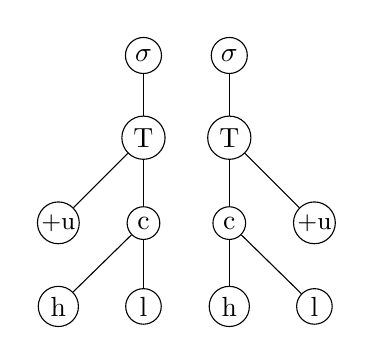
\begin{tikzpicture} [baseline = (y1.base)]
\matrix (m) [matrix of nodes, column sep = 1.5em, row sep = 1.5em]{
& \node[draw,circle, inner sep =2pt](x1){$\sigma$};  &  \node[draw,circle, inner sep =2pt](x2){$\sigma$};  \\
& \node[draw,circle, inner sep =2pt](y1){T}; &   \node[draw,circle, inner sep =2pt](y2){T}; \\
\node[draw,circle, inner sep =.5pt](z1){\small +u}; & \node[draw,circle, inner sep =2pt](z2){c}; &   \node[draw,circle, inner sep =2pt](z3){c}; & \node[draw,circle, inner sep =.5pt](z4){\small +u}; \\
\node[draw,circle, inner sep =2pt](t1){h}; & \node[draw,circle, inner sep =2pt](t2){l}; &  \node[draw,circle, inner sep =2pt](t3){h}; & \node[draw,circle, inner sep =2pt](t4){l}; \\
};
\draw (x1) -- (y1);
\draw (x2) -- (y2);
\draw (z1) -- (y1);
\draw (z2) -- (y1);
\draw (z2) -- (t1);
\draw (z2) -- (t2);
\draw (y2) -- (z3);
\draw (y2) -- (z4);
\draw (z3) -- (t3);
\draw (t4) -- (z3);
\end{tikzpicture}
\hspace{.3cm}
$\rightarrow$
\hspace{.3cm}
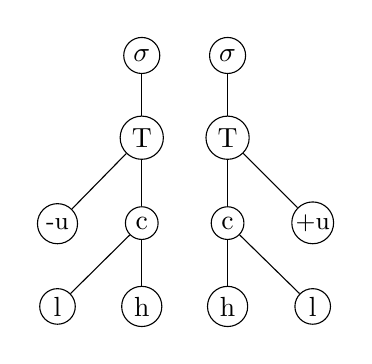
\begin{tikzpicture} [baseline = (y1.base)]
\matrix (m) [matrix of nodes, column sep = 1.5em, row sep = 1.5em]{
& \node[draw,circle, inner sep =2pt](x1){$\sigma$};  &  \node[draw,circle, inner sep =2pt](x2){$\sigma$};  \\
& \node[draw,circle, inner sep =2pt](y1){T}; &   \node[draw,circle, inner sep =2pt](y2){T}; \\
\node[draw,circle, inner sep =2pt](z1){\small -u}; & \node[draw,circle, inner sep =2pt](z2){c}; &   \node[draw,circle, inner sep =2pt](z3){c}; & \node[draw,circle, inner sep =.5pt](z4){\small +u}; \\
\node[draw,circle, inner sep =2pt](t1){l}; & \node[draw,circle, inner sep =2pt](t2){h}; &  \node[draw,circle, inner sep =2pt](t3){h}; & \node[draw,circle, inner sep =2pt](t4){l}; \\
};
\draw (x1) -- (y1);
\draw (x2) -- (y2);
\draw (z1) -- (y1);
\draw (z2) -- (y1);
\draw (z2) -- (t1);
\draw (z2) -- (t2);
\draw (y2) -- (z3);
\draw (y2) -- (z4);
\draw (z3) -- (t3);
\draw (t4) -- (z3);
\end{tikzpicture}
\hspace{.3cm}
$\equiv$ /HM.HM/$\mapsto$[ML.HM]
\end{center}
\begin{center}
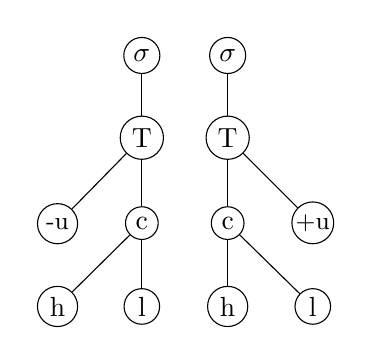
\begin{tikzpicture} [baseline = (y1.base)]
\matrix (m) [matrix of nodes, column sep = 1.5em, row sep = 1.5em]{
& \node[draw,circle, inner sep =2pt](x1){$\sigma$};  &  \node[draw,circle, inner sep =2pt](x2){$\sigma$};  \\
& \node[draw,circle, inner sep =2pt](y1){T}; &   \node[draw,circle, inner sep =2pt](y2){T}; \\
\node[draw,circle, inner sep =2pt](z1){\small -u}; & \node[draw,circle, inner sep =2pt](z2){c}; &   \node[draw,circle, inner sep =2pt](z3){c}; & \node[draw,circle, inner sep =.5pt](z4){\small +u}; \\
\node[draw,circle, inner sep =2pt](t1){h}; & \node[draw,circle, inner sep =2pt](t2){l}; &  \node[draw,circle, inner sep =2pt](t3){h}; & \node[draw,circle, inner sep =2pt](t4){l}; \\
};
\draw (x1) -- (y1);
\draw (x2) -- (y2);
\draw (z1) -- (y1);
\draw (z2) -- (y1);
\draw (z2) -- (t1);
\draw (z2) -- (t2);
\draw (y2) -- (z3);
\draw (y2) -- (z4);
\draw (z3) -- (t3);
\draw (t4) -- (z3);
\end{tikzpicture}
\hspace{.3cm}
$\rightarrow$
\hspace{.3cm}
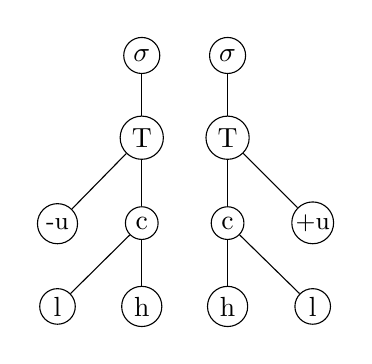
\begin{tikzpicture} [baseline = (y1.base)]
\matrix (m) [matrix of nodes, column sep = 1.5em, row sep = 1.5em]{
& \node[draw,circle, inner sep =2pt](x1){$\sigma$};  &  \node[draw,circle, inner sep =2pt](x2){$\sigma$};  \\
& \node[draw,circle, inner sep =2pt](y1){T}; &   \node[draw,circle, inner sep =2pt](y2){T}; \\
\node[draw,circle, inner sep =2pt](z1){\small -u}; & \node[draw,circle, inner sep =2pt](z2){c}; &   \node[draw,circle, inner sep =2pt](z3){c}; & \node[draw,circle, inner sep =.5pt](z4){\small +u}; \\
\node[draw,circle, inner sep =2pt](t1){l}; & \node[draw,circle, inner sep =2pt](t2){h}; &  \node[draw,circle, inner sep =2pt](t3){h}; & \node[draw,circle, inner sep =2pt](t4){l}; \\
};
\draw (x1) -- (y1);
\draw (x2) -- (y2);
\draw (z1) -- (y1);
\draw (z2) -- (y1);
\draw (z2) -- (t1);
\draw (z2) -- (t2);
\draw (y2) -- (z3);
\draw (y2) -- (z4);
\draw (z3) -- (t3);
\draw (t4) -- (z3);
\end{tikzpicture}
\hspace{.3cm}
$\equiv$ /ML.HM/$\mapsto$[ML.HM]
\end{center}
\begin{center}
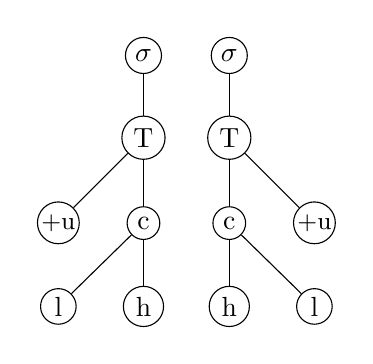
\begin{tikzpicture} [baseline = (y1.base)]
\matrix (m) [matrix of nodes, column sep = 1.5em, row sep = 1.5em]{
& \node[draw,circle, inner sep =2pt](x1){$\sigma$};  &  \node[draw,circle, inner sep =2pt](x2){$\sigma$};  \\
& \node[draw,circle, inner sep =2pt](y1){T}; &   \node[draw,circle, inner sep =2pt](y2){T}; \\
\node[draw,circle, inner sep =.5pt](z1){\small +u}; & \node[draw,circle, inner sep =2pt](z2){c}; &   \node[draw,circle, inner sep =2pt](z3){c}; & \node[draw,circle, inner sep =.5pt](z4){\small +u}; \\
\node[draw,circle, inner sep =2pt](t1){l}; & \node[draw,circle, inner sep =2pt](t2){h}; &  \node[draw,circle, inner sep =2pt](t3){h}; & \node[draw,circle, inner sep =2pt](t4){l}; \\
};
\draw (x1) -- (y1);
\draw (x2) -- (y2);
\draw (z1) -- (y1);
\draw (z2) -- (y1);
\draw (z2) -- (t1);
\draw (z2) -- (t2);
\draw (y2) -- (z3);
\draw (y2) -- (z4);
\draw (z3) -- (t3);
\draw (t4) -- (z3);
\end{tikzpicture}
\hspace{.3cm}
$\rightarrow$
\hspace{.3cm}
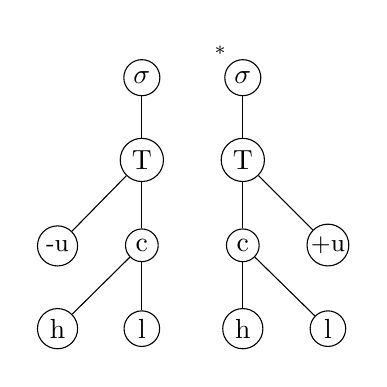
\begin{tikzpicture} [baseline = (y1.base)]
\matrix (m) [matrix of nodes, column sep = 1.5em, row sep = 1.5em]{
& \node[draw,circle, inner sep =2pt](x1){$\sigma$};  &  \node[draw,circle, inner sep =2pt, label={[label distance=-3pt] above left:\scriptsize *}](x2){$\sigma$};  \\
& \node[draw,circle, inner sep =2pt](y1){T}; &   \node[draw,circle, inner sep =2pt](y2){T}; \\
\node[draw,circle, inner sep =2pt](z1){\small -u}; & \node[draw,circle, inner sep =2pt](z2){c}; &   \node[draw,circle, inner sep =2pt](z3){c}; & \node[draw,circle, inner sep =.5pt](z4){\small +u}; \\
\node[draw,circle, inner sep =2pt](t1){h}; & \node[draw,circle, inner sep =2pt](t2){l}; &  \node[draw,circle, inner sep =2pt](t3){h}; & \node[draw,circle, inner sep =2pt](t4){l}; \\
};
\draw (x1) -- (y1);
\draw (x2) -- (y2);
\draw (z1) -- (y1);
\draw (z2) -- (y1);
\draw (z2) -- (t1);
\draw (z2) -- (t2);
\draw (y2) -- (z3);
\draw (y2) -- (z4);
\draw (z3) -- (t3);
\draw (t4) -- (z3);
\end{tikzpicture}
\hspace{.3cm}
$\equiv$ /MH.HM/$\mapsto$*[LM.HM]
\end{center}
\begin{center}
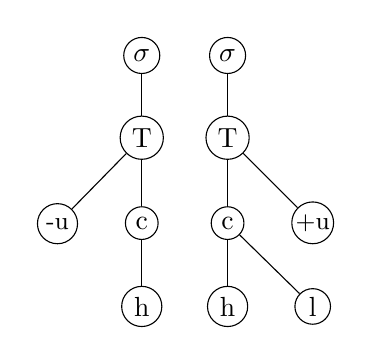
\begin{tikzpicture} [baseline = (y1.base)]
\matrix (m) [matrix of nodes, column sep = 1.5em, row sep = 1.5em]{
& \node[draw,circle, inner sep =2pt](x1){$\sigma$};  &  \node[draw,circle, inner sep =2pt](x2){$\sigma$};  \\
& \node[draw,circle, inner sep =2pt](y1){T}; &   \node[draw,circle, inner sep =2pt](y2){T}; \\
\node[draw,circle, inner sep =2pt](z1){\small -u}; & \node[draw,circle, inner sep =2pt](z2){c}; &   \node[draw,circle, inner sep =2pt](z3){c}; & \node[draw,circle, inner sep =.5pt](z4){\small +u}; \\
& \node[draw,circle, inner sep =2pt](t2){h}; &  \node[draw,circle, inner sep =2pt](t3){h}; & \node[draw,circle, inner sep =2pt](t4){l}; \\
};
\draw (x1) -- (y1);
\draw (x2) -- (y2);
\draw (z1) -- (y1);
\draw (z2) -- (y1);
\draw (z2) -- (t2);
\draw (y2) -- (z3);
\draw (y2) -- (z4);
\draw (z3) -- (t3);
\draw (t4) -- (z3);
\end{tikzpicture}
\hspace{.3cm}
$\rightarrow$
\hspace{.3cm}
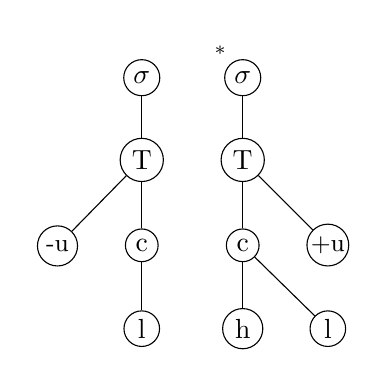
\begin{tikzpicture} [baseline = (y1.base)]
\matrix (m) [matrix of nodes, column sep = 1.5em, row sep = 1.5em]{
& \node[draw,circle, inner sep =2pt](x1){$\sigma$};  &  \node[draw,circle, inner sep =2pt, label={[label distance=-3pt] above left:\scriptsize *}](x2){$\sigma$};  \\
& \node[draw,circle, inner sep =2pt](y1){T}; &   \node[draw,circle, inner sep =2pt](y2){T}; \\
\node[draw,circle, inner sep =2pt](z1){\small -u}; & \node[draw,circle, inner sep =2pt](z2){c}; &   \node[draw,circle, inner sep =2pt](z3){c}; & \node[draw,circle, inner sep =.5pt](z4){\small +u}; \\
& \node[draw,circle, inner sep =2pt](t2){l}; &  \node[draw,circle, inner sep =2pt](t3){h}; & \node[draw,circle, inner sep =2pt](t4){l}; \\
};
\draw (x1) -- (y1);
\draw (x2) -- (y2);
\draw (z1) -- (y1);
\draw (z2) -- (y1);
\draw (z2) -- (t2);
\draw (y2) -- (z3);
\draw (y2) -- (z4);
\draw (z3) -- (t3);
\draw (t4) -- (z3);
\end{tikzpicture}
\hspace{.3cm}
$\equiv$ /M.HM/$\mapsto$*[L.HM]
\end{center}
The definition of the transduction will only evaluate to true for maps which contain a non-final, high-falling contour. 
\bibliographystyle{apalike}
\bibliography{references}
\end{document}